\subsection{HTB02 - Magic}
\subsubsection{Escaneo}
En la fase de escaneo mediante la herramienta “Nmap” se observó que se encontraban 2 puertos abiertos, el puerto 22 del servicio SSH y el puerto 80 usando como servidor Apache.
\begin{figure}[H]
    \centering
    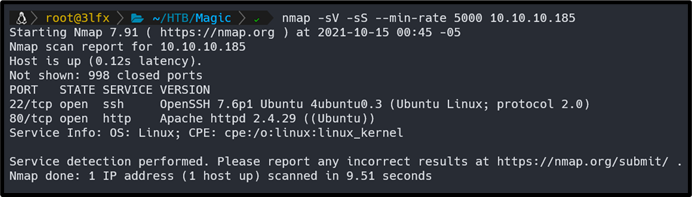
\includegraphics[width=0.99\textwidth]{imagenes/scanmag.png}
    \caption{Escaneo de puertos Magic}
\end{figure}
\subsubsection{Análisis de Vulnerabilidades y debilidades}
Se procedió a analizar el sitio web de la máquina, teniendo vista de varias imágenes.
\begin{figure}[H]
    \centering
    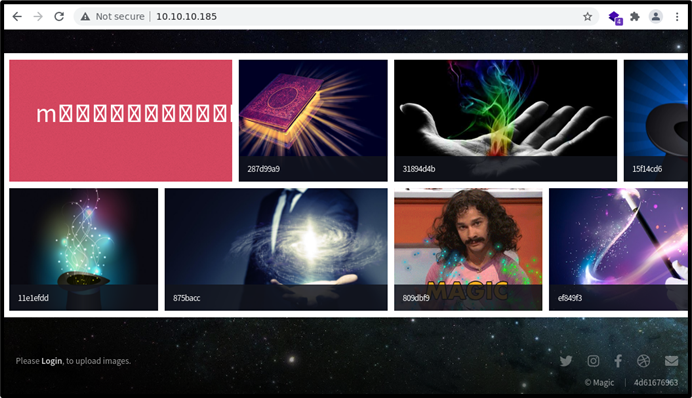
\includegraphics[width=0.99\textwidth]{imagenes/pagmag.png}
    \caption{Página web Magic}
\end{figure}
En la parte de abajo se observa que se necesita iniciar sesión para subir imágenes. Por ello se procede a dirigirse al Login teniendo el siguiente formulario.
\begin{figure}[H]
    \centering
    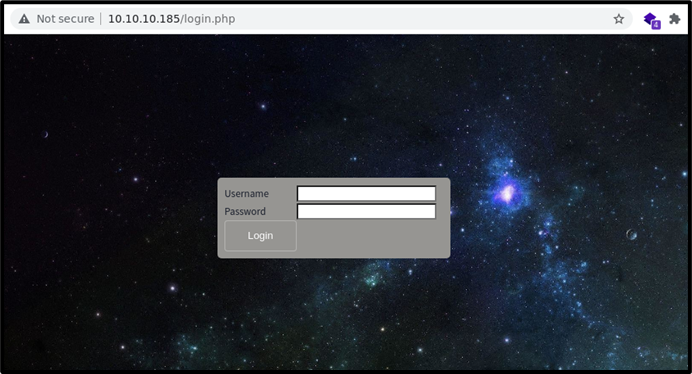
\includegraphics[width=0.9\textwidth]{imagenes/logmag.png}
    \caption{Servicio Login en sitio web Magic}
\end{figure}
Se intentó algunos usuarios y contraseñas genéricas sin tener éxito donde se notificaba que el usuario o contraseña era incorrecto, lo siguiente a realizar fue intentar una inyección SQL teniendo como parámetro de username (’ 1=1;) y en la contraseña cualquier valor, después de ello se recarga la página, pero sin indicarnos que el usuario o contraseña era incorrecto, lo que indica que si es vulnerable a inyección SQL (VU02, DE03). Continuando con la inyección SQL se realizó utilizando para acceder al usuario “admin” al usar como parámetro de username (admin’;), esto permite acceder a la página de “upload.php” como se puede ver en la siguiente imagen.
\begin{figure}[H]
    \centering
    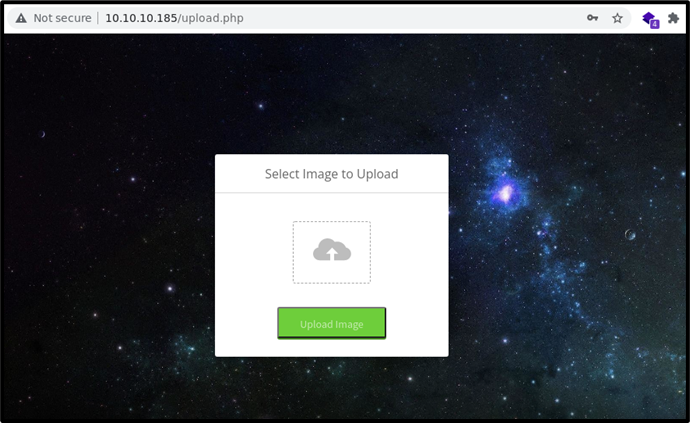
\includegraphics[width=0.9\textwidth]{imagenes/submag.png}
    \caption{Página para subida de imágenes en Magic}
\end{figure}
\subsubsection{Explotación}
Una vez teniendo acceso para subir imágenes, se procede a la fase de explotación donde al tener permitido el subido de archivos, se procederá a tener acceso mediante una Reverse Shell. Se intentó subir un archivo con la terminación “.php”, pero no permite otros archivos que no sean imágenes, también se hizo la prueba cambiándole la extensión, pero el servidor valida los metadatos para confirmar que sean imágenes (DE04).

Por ello se incrusto una carga útil a una imagen real para realizar la Reverse Shell, esto se hizo con la herramienta “exiftool” agregando la carga útil en como comentario de la imagen y se cambió la extensión a “.php.jpg”.
\begin{figure}[H]
    \centering
    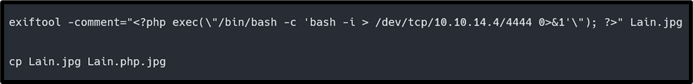
\includegraphics[width=0.99\textwidth]{imagenes/inyima.png}
    \caption{Inyección de código malicioso en imagen}
\end{figure}
Se procede subiendo el archivo y es aceptado por el servidor, ahora se consulta la imagen en la ruta “/images/uploads/” donde estaban todas las demás imágenes que aparecen en la página principal. Esto genera el acceso a la máquina como “www-data” como se puede apreciar en la siguiente imagen.
\begin{figure}[H]
    \centering
    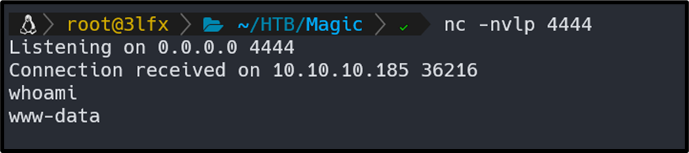
\includegraphics[width=0.8\textwidth]{imagenes/acwma.png}
    \caption{Acceso como ``www-data” en máquina Magic}
\end{figure}
\subsubsection{Escalamiento de Privilegios}
Para el escalamiento de privilegios se revisó el directorio “Magic”, abriendo el archivo “db.php5” donde se encontró un usuario y contraseña de base de datos como se muestra en la siguiente imagen (DE01).
\begin{figure}[H]
    \centering
    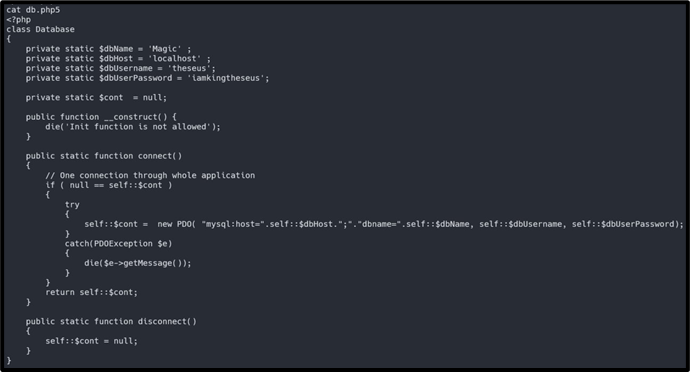
\includegraphics[width=0.99\textwidth]{imagenes/conarma.png}
    \caption{Contraseña en archivo de configuración en máquina Magic}
\end{figure}
Se intentó acceder a la máquina como “Theseus” con esa contraseña, pero no se tuvo éxito, por ello se intenta usar el comando “mysql” pero no existe, luego buscando otro comando para ejecutar se intentó “mysqldump” para extraer la información de la base de datos.
\begin{figure}[H]
    \centering
    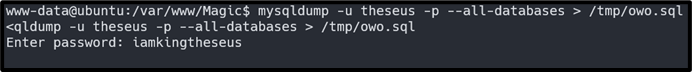
\includegraphics[width=0.99\textwidth]{imagenes/basemag.png}
    \caption{Extracción de tablas de base de datos en Magic}
\end{figure}
Una vez realizado el proceso anterior, se procede a leer el archivo generado, encontrando allí otra contraseña como se muestra en la siguiente imagen.
\begin{figure}[H]
    \centering
    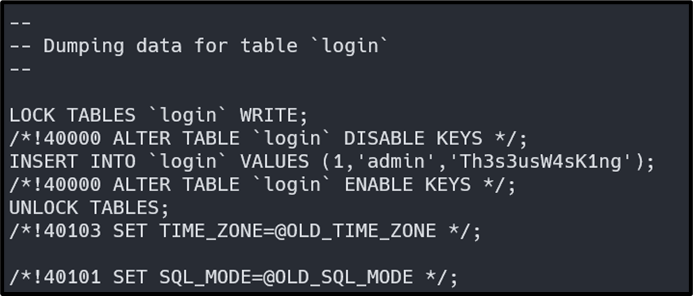
\includegraphics[width=0.9\textwidth]{imagenes/tabmag.png}
    \caption{Contraseña en base de datos Magic}
\end{figure}
Con esa contraseña encontrada se procede a intentar acceder mediante el usuario Theseus y se consigue exitosamente, como prueba se tiene la siguiente imagen.
\begin{figure}[H]
    \centering
    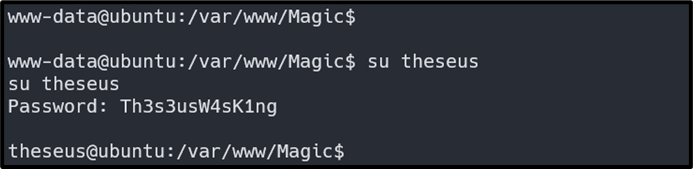
\includegraphics[width=0.99\textwidth]{imagenes/acthe.png}
    \caption{Acceso a usuario Theseus en Magic}
\end{figure}
Se procede a listar los archivos con permiso SUID mostrando esta lista en la siguiente imagen.
\begin{figure}[H]
    \centering
    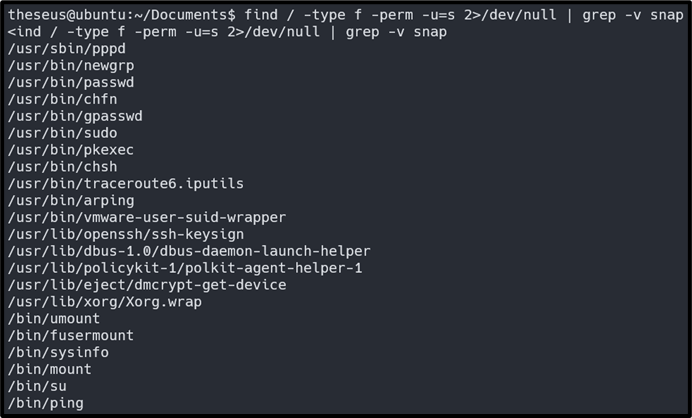
\includegraphics[width=0.99\textwidth]{imagenes/listsuma.png}
    \caption{Listado de archivos con permiso SUID en Magic}
\end{figure}
Del proceso anterior se observa el archivo “sysinfo” del que se procederá a analizar su función. A partir de los caracteres imprimibles se encuentra que ejecuta ciertos comandos .
\begin{figure}[H]
    \centering
    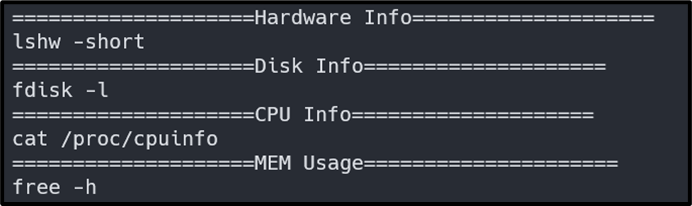
\includegraphics[width=0.9\textwidth]{imagenes/sysin.png}
    \caption{Comandos que ejecuta ``sysinfo''}
\end{figure}
Se encontró información de este programa que cuenta con una vulnerabilidad, por ello se procederá a realizar un secuestro de PATH para escalar privilegios (VU03, DE07).

Lo siguiente a realizar es crear un archivo “lshw” con la que se obtendrá una Reverse Shell, y pasar el archivo desde la máquina atacante hacia la victima mediante el levantamiento de un servidor HTTP con Python.
\begin{figure}[H]
    \centering
    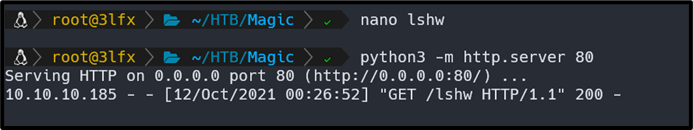
\includegraphics[width=0.9\textwidth]{imagenes/seratma.png}
    \caption{Servidor HTTP en máquina atacante}
\end{figure}
En la máquina víctima se procede a descargar el archivo creado y se le cambia los permisos de ejecución para luego proceder a agregar el directorio “/tmp” al PATH lo que permitirá la ejecución de archivo creado mediante el binario “sysinfo”.
\begin{figure}[H]
    \centering
    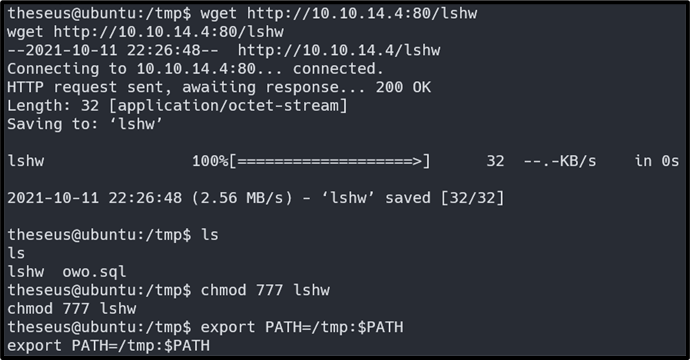
\includegraphics[width=0.9\textwidth]{imagenes/armalmag.png}
    \caption{Configuración de archivo malicioso en Magic}
\end{figure}
Lo siguiente a realizar tener en escucha el puerto indicado en el archivo “lshw” y después ejecutar el comando “sysinfo”, como resultado se obtiene conexión a la máquina objetivo como el usuario “root”.
\begin{figure}[H]
    \centering
    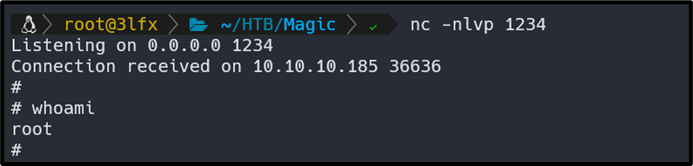
\includegraphics[width=0.9\textwidth]{imagenes/acrootmag.png}
    \caption{Acceso al usuario root en máquina Magic}
\end{figure}
\subsubsection{Post-explotación}
En la fase de post-explotación se procede a extraer las credenciales de los usuarios pertenecientes a la máquina “Magic”, teniendo de prueba la siguiente imagen.
\begin{figure}[H]
    \centering
    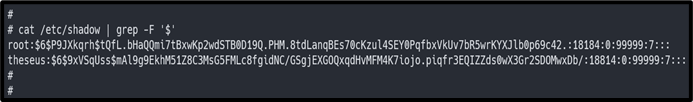
\includegraphics[width=0.99\textwidth]{imagenes/hashmag.png}
    \caption{Extracción de contraseñas en formato hash de Magic}
\end{figure}
\subsubsection{Recomendaciones de mitigación}
Para mitigar las vulnerabilidades y debilidades encontradas en la máquina Magic, se recomienda lo siguiente:
\begin{itemize}
    \item Neutralizar correctamente los elementos especiales al momento de realizar comandos SQL en el servicio Login, con la finalidad de evitar el acceso no autorizado mediante la inyección SQL en el sitio web.
    \item Realizar un mejor control de archivos permitidos para cargar al sitio web para evitar que se suba imágenes con código malicioso que permita el acceso al sistema.
    \item No utilizar herramientas como “sysinfo”, que se ejecutan con altos privilegios, lo que permitiría a un usuario el escalamiento de privilegios, o en su defecto configurarlo para que solo se permita su ejecución por el usuario “root”.
\end{itemize}